\documentclass{article}

\usepackage{caption,color,fancyvrb,subfig}
\usepackage{code,algorithmic,algorithm}
\usepackage{graphicx,epsfig}
\usepackage{amsmath,amsthm,amsfonts}
\usepackage{amssymb}
\usepackage{setspace}
\usepackage{bibentry}

\nobibliography{prelim}

\textwidth = 6.5 in
\textheight = 9 in
\oddsidemargin = 0.0 in
\evensidemargin = 0.0 in
\topmargin = 0.0 in
\headheight = 0.0 in
\headsep = 0.0 in
\parskip = 0.12in
\parindent = 0.0in


\def\inv{^{-1}}



\begin{document}

\begin{titlepage}
\begin{center}

\textsc{\huge \bfseries \sc{Responsive Consistency in Heterogenous,}}\\
\textsc{\huge \bfseries \sc{Wide Area Distributed Storage Systems}}\\[1.0cm]

\emph{A prospectus submitted in partial fulfillment of the degree of Doctor of
Philosophy}\\[5.5cm]

\textsc{\large DRAFT}\\
\emph{October 11, 2016}\\[2.0cm]

\emph{Preliminary Oral Examination for}\\
\textsc{\large Benjamin Bengfort}\\[2.0cm] % [4.0cm]
\emph{Advisor:} \\
\textsc{Dr. Peter J. Keleher}\\[.5cm]
\emph{Committee Members:}\\
\textsc{Dr. Bobby Bhattacharjee}\\
\textsc{Dr. Dave Levin}\\
\textsc{Dr. Neil Spring}\\[4.0cm]

{\bfseries Department of Computer Science}\\
{\bfseries University of Maryland, College Park, MD 20742}\\
{\bfseries December 9, 2016}
\vfill

\end{center}
\end{titlepage}

\newpage
\thispagestyle{empty}
\mbox{}


\newpage
\setcounter{page}{1}
\onehalfspacing
\begin{abstract}

Data-oriented consistency is not a discrete set of various levels, weak, eventual, causal, strong etc. but rather a continuum that can be adapted in response to environmental conditions. Recent studies of consistency have focused on data center environments which are low latency, high bandwidth, and generally stable; and as a result data distribution involves a relatively small network of devices. I propose to study consistency in a user-oriented context composed of heterogenous devices (mobile phones, desktops, laptops, cloud storage) that can be mobile, creating a network topology of highly variable latency with routine failure and whose networks are larger than typically studied - dozens to hundreds of replica servers.

Our primary context will be a file system that exposes close-to-open consistency and tracks writes to individual objects as a sequence of versions structured as a tree. We consider strong consistency to be a linear sequence of ordered version numbers and inconsistencies to be the presence of forks, misordering, duplicates, or omissions in the version sequence (in order of severity). Additionally we consider the availability of such a system and recognize that enforcement of a linear ordering leads to high latency making the system unusable.

I propose that consistency is primarily related to the network environment as much as it is related to the implemented protocol and as a result, that it can respond the the environment. By creating a system that has a strong central core that maintains a globally consistent view and allowing other replica servers to be flexible I hypothesize that the system will be more consistent than its homogeneous counterparts reducing the number of forks, misordering, duplicates, and omissions as well increasing the throughput and availability of accesses in the system. I propose two primary mechanisms to make this happen:

\begin{enumerate}
    \item \textbf{Federated Consistency}: allow multiple consistency models for different replica servers, integrating over different aspects: temporal, spatial, and synchronization to create a flexible topology of devices with different characteristics and nodes.
    \item \textbf{Hierarchical Consensus}: distribute consensus decisions of sequential ordering in order to make stronger consistency more available.
\end{enumerate}

The experimentation on and development of multi-modal replication protocols via a holistic view will have a large impact in both the data center context as well as in personal distributed file systems.

\end{abstract}
\setstretch{.5}

\newpage
\setcounter{tocdepth}{2}
\tableofcontents

\newpage
\listoffigures

\newpage
\onehalfspacing

%\begin{figure}[!h]
%\begin{center}
%\begin{verbatim}
%/* Sample code snippet */
%\end{verbatim}
%\end{center}
%\caption{Code snippet caption}
%\label{fig:sample_code}
%\end{figure}

% \begin{figure}[!h]
%     \centering
%         \includegraphics[width=.9\textwidth]{figures/figure.png}
%         \caption{Figure caption}
%         \label{fig:label}
% \end{figure}

\section{Introduction}

The rise of virtualized, on-demand computing resources and cloud computing has dramatically shifted the focus of research on consistency in distributed storage systems away from networked file systems toward geographically distributed database management systems, particularly key-value storage. These types of data systems benefit from low-latency, high-bandwidth connections where failure is common due to the magnitude of resources rather than inherent instability. Because most distribution protocols that provide consistency guarantees are dependent on timing parameters related to the latency of messages, it can be shown that consistency is more dependent on network environment than specific protocols. As a result, ``eventually consistent'' \cite{vogels_eventually_2009} systems are said to be consistent enough for most workloads given some probabilistic bounding of staleness \cite{bailis_quantifying_2014,bermbach_eventual_2011,bailis_probabilistically_2012}. This has led consistency research towards investigating stronger forms of eventual consistency, primarily building upon Dynamo \cite{decandia_dynamo:_2007} and Cassandra \cite{lakshman_cassandra:_2010} as reference implementations. Alternatively, research into ensuring strong, sequential consistency in this environment has led to systems like Spanner \cite{corbett_spanner:_2013} which uses atomic and GPS clocks to ensure ``TrueTime'' for sequential ordering or a small number of master nodes that implement consensus algorithms \cite{lamport_paxos_2001,ongaro_search_2014} for locking or ordering \cite{kraska_mdcc:_2013}.

Unfortunately the focus on data center consistency has led to a centralized approach to data storage, forcing a modality where devices must connect to the cloud for file replication even when files exist in the local area \cite{drago_inside_2012}. Although this allows systems to ignore annoyances such as local network configuration and decentralized consistency it does present unnecessary overhead in terms of cost and latency. More pernicious, perhaps, is that users must now buy-in and store their data with a single provider that could go out of business or be hacked leading to research in replicating local data with multiple untrusted cloud stores \cite{zhang_viewbox:_2014,feldman_sporc:_2010}. Finally, there are more devices than ever before connecting to storage applications, partially because users have multiple, heterogenous devices from wearables to workstations and partially because of the advent of the Internet of Things \cite{miorandi_internet_2012}.

We propose to study consistency in user-oriented networks: heterogenous, mobile, variable-latency, and partition-prone topologies with multiple devices and users. Because of the user-centric nature of this research, we further propose the study of a file system as the primary data storage application in such networks. File systems must be highly available such that a user does not notice any delay due to coordination but must also have strong consistency such that any conflicts are presented to the user as soon as possible. To that end, our consistency model must be \textit{responsive} to the network environment providing flexibility when the network is unavailable or laggy and providing strong consistency guarantees when stable connections exist.

Our approach therefore focuses on two primary techniques: the \textit{federation} of weak but available consistency mechanisms with sequential consistency by consensus and the \textit{hierarchical} clustering of quorums so as to minimize conflict by creating localities of interest with global guarantees. We hypothesize that the integration of multi-modal consistency will lead to higher availability than strong consistency models but provide stronger guarantees than eventually consistent systems. We will quantitatively demonstrate the efficacy of such a system by comparing it to homogenous systems with similar sizes and topologies and measuring the number of inconsistencies and amount of latency in both simulation and a real world implementation.

\section{Related Work}

Our work stems from open questions related to data-centric consistency models, previously thought of as discrete levels but now viewed as a continuum along the dimensions of ordering and staleness \cite{bermbach_consistency_2013}. In the first part of this section, I will review and identify various consistency models. There are two primary mechanisms to replicate data with specific consistency: anti-entropy combined with various policies and centralization via consensus, each of which I will explore in detail. Finally I will contextualize our work with consistency rationing and hierarchical models of consensus previously put forward as well as a specific look at related systems.

\subsection{Consistency}

% Should I review the client-centric consistency models

Our consistency model is a \textit{data-centric} model which concerns two primary dimensions: ordering and staleness. Given that every replica maintains a local log of accesses with respect to some abstract total ordering based on the sequence of version numbers and potentially concurrent operations, we can define those dimensions as follows:

\begin{enumerate}
    \item \textit{Ordering} refers to how closely individual logs adhere to the abstract global ordering. A \textit{strict ordering} requires every single log to be exactly the same whereas weaker ordering allows some divergence in the order writes are stored in the log.
    \item \textit{Staleness} refers to how far behind the latest global version a local log is and can be either expressed by the visibility latency of replicating a version to all replicas or simply by how many versions the latest is behind by.
\end{enumerate}

Most data-centric consistency models do not consider staleness but instead refer to the strictness of ordering guarantees and the method by which updates are applied to the state of the replica. Indeed, ordering strictness can lead to to increased staleness because writes cannot be accepted until they have fulfilled their dependencies first, creating further delay. Our consistency model considers instead the primary symptom of stale reads and writes: \textit{forks}.

\begin{description}
    \item[\textbf{Fork}] A fork occurs when two replicas concurrently write a new version to the same parent object as shown in Figure \ref{fig:forks}. Forks introduce inconsistency because there are now two potential orderings of updates to the log, but forks are primarily the symptom of staleness; e.g. the second writer wrote to a stale version of the object.
\end{description}

There are two primary causes of forks: concurrent accesses by multiple replicas and stale reads. The former is distinguished from the latter only if the possibility of synchronization could have occurred. From the point of view of the system, they are identical causes. Forks can branch to arbitrary lengths as replicas continue to write to their latest local copies, however when synchronization occurs a decision as to which ordering of writes is correct must occur.

\begin{figure}
    \centering
        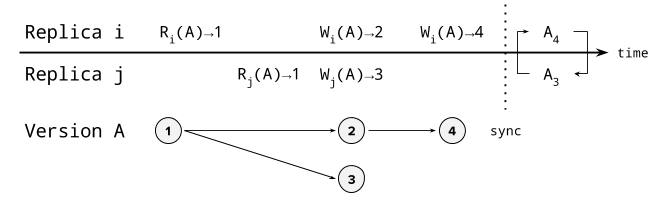
\includegraphics[width=.9\textwidth]{figures/forks}
        \caption{Forks branch sequentially ordered version numbers}
        \label{fig:forks}
\end{figure}

With this context and consistency model in mind, we can now identify several consistency models in order of increasing ordering strictness and define how each model's correctness criteria responds in the face of forks.

\subsubsection{Weak Consistency}

A weakly consistent system makes no guarantees whatsoever about the relationship of local vs. remote writes and whether or not any given update will become visible \cite{vogels_eventually_2009}. Weak consistency is often described as ``replicas might get lucky and become consistent'' and in fact a weakly consistent implementation may not have a synchronization protocol whatsoever \cite{bermbach_consistency_2013}.

\subsubsection{Eventual Consistency}

Eventual consistency is primarily concerned with the final state of all logs in the system given some period of quiescence that allows the system to converge. In this case, all replicas, no matter their log ordering, should have identical final versions for all objects in the namespace. This suggests that eventual consistency requires some \textit{anti-entropy} mechanism to propagate writes and a policy to handle convergence \cite{terry_managing_1995}. Eventual consistency is very popular for NoSQL databases and hosted distributed storage services \cite{decandia_dynamo:_2007,lakshman_cassandra:_2010} because it favors an optimistic approach to consistency: in most systems conflicts are rare, and if something does go wrong, conflict resolution is up to the application layer. In practice, most applications can handle some inconsistency and moreover the small inconsistency windows due to low latencies in cloud data centers make such conflicts rare and short-lived enough to be worth the risk \cite{bailis_quantifying_2014}.

Eventual consistency implemented by a \textit{last writer wins} policy simply accepts all writes so long as they are more recent than the latest local versions. Eventual reads and writes are always performed locally, and therefore with little performance overhead. Eventual allows forks to occur and moreover allows individual replica logs to have wholly different orderings so long as the last version for each object is in the same given no writes for a long enough period of time. As a result, the latest version of an object may alternate between writes to competing forks (a fairly weak semantic) and in this case, it is up to the application to detect the inconsistency. However, Eventual logs do have one important property - for each object, every write in the log is ordered in a monotonically increasing fashion.

\subsubsection{Causal Consistency}

In causal consistency all writes that have causal relationships must have those dependencies satisfied, e.g. inserted into the log before that write can become visible. Therefore, even though a write might have been propagated to another replica server it cannot be read until all of its dependencies have also been propagated. Causal consistency can increase staleness particularly when implicit or potential causality creates large dependency graphs that must be resolved before writes can be applied \cite{lloyd_dont_2011}. This can be managed by allowing the application to explicitly specify the dependencies for each write \cite{bailis_potential_2012}.

\subsubsection{Sequential Consistency}

Sequential consistency is a strong consistency model that requires that all replicas have the exact same ordering of their logs, such that all writes by all clients are appended in the same exact order \cite{attiya_sequential_1994}. Sequential consistency is not strict in that it does not make guarantees about staleness (or the ordering of reads) but does require that all writes become visible in the same order \cite{bermbach_consistency_2013}. Sequentially consistency is typically implemented with consensus algorithms such as Paxos \cite{lamport_fast_2006} or Raft \cite{ongaro_search_2014} that coordinate logs by defining a transitive, global ordering for all conflicts. Alternatively, sequential consistency and can be implemented with warranties -- time based assertions about a group of objects that must be met on all replicas before the assertions expired \cite{liu_warranties_2014}.

\subsubsection{Linearizability}

Linearizability is the strongest form of consistency; not only must all write operations occur in sequence, but all operations including reads must be ordered chronologically \cite{herlihy_linearizability:_1990}. A consensus algorithm alone cannot implement linearizability and instead some distributed locking mechanism is required. For example a consensus algorithm can be adapted to instead of making decisions about the total ordering of conflicting writes, granting or releasing locks from requestors, however this opens up the potential for deadlock and extremely poor performance, defeating the purposes of replication in the first place! Data center environments that don't have to deal with issues of clock skew by using super precise atomic and GPS clocks can use precise time measurements to enable a distributed two phase commit protocol \cite{corbett_spanner:_2013}, however every replica is required to have such a time piece, which is not practical for heterogenous topologies.

\subsection{Anti-Entropy}

Eventual consistency is implemented by periodic \textit{anti-entropy} sessions that converge replicas towards the same state (e.g. reducing entropy, the divergence between the states of individual replicas) \cite{kempe_gossip-based_2003, karp_randomized_2000}. On a routine interval, specified by the \texttt{anti-entropy delay} timing parameter, a replica will randomly select one of the other replicas in the system and send a \texttt{Gossip} message that contains the latest version of all objects in the replica's local log.

\subsection{Consensus}

Consensus algorithms are generally variations of the Paxos algorithm \cite{lamport_paxos_2001} and more specifically the Fast Paxos implementation \cite{lamport_fast_2006}. For example S-Paxos \cite{biely_s-paxos:_2012} attempts to distribute the workload of the leader (similar to hierarchical consensus), Multi-Paxos \cite{camargos_multicoordinated_2007} allows multiple leaders per round, Flexible Paxos \cite{2016arXiv160806696H} allows for multiple quorum intersections, and Egalitarian Paxos \cite{moraru_egalitarian_2012,moraru_there_2013} allow fast and slow track voting.

However, Paxos has been shown to be very difficult to correctly implement and verify \cite{chandra_paxos_2007} and although attempts have been made to highlight the practicality of a subset of the Paxos guarantees \cite{mazieres_paxos_2007} it has been shown that Paxos is not understandable. To that end, we have used the Raft consensus protocol \cite{ongaro_search_2014, howard_raft_2015} as our primary consensus implementation.

\subsection{Consistency Rationing and Hybridization}

One of the earliest attempts to hybridize weak and strong consistency was a model for parallel programming on shared memory systems by Agrawal et al \cite{agrawal_mixed_1994}. This model allowed programmers to relax strong consistency in certain contexts with causal memory or pipelined random access in order to improve parallel performance of applications. Per-operation consistency was extended to distributed storage by the RedBlue consistency model of Li et al \cite{li_making_2012}. Here, replication operations are broken down into small, commutative suboperations that are classified as red (must be executed in the same order on all replicas) or blue (execution order can vary from site to site), so long as the dependencies of each suboperation are maintained. The consistency model is therefore global, specified by the red/blue ordering and can be adapted by redefining the ratio of red to blue operations, e.g. all blue operations is an eventually consistent system and all red is sequential.

The next level above per-operation consistency hybridization is called \textit{consistency rationing} wherein individual objects or groups of objects have different consistency levels applied to them to create a global quality of service guarantee. Kraska et al. \cite{kraska_consistency_2009} initially proposed consistency rationing be on a per-transaction basis by classifying objects in three tiers: eventual, adaptable, and linearizable. Objects in the first and last groups were automatically assigned transaction semantics that maintained that level of consistency; however objects assigned the adaptable categorization had their consistency policies switched at runtime based on a cost function that either minimized time or write costs depending on user preference. This allowed consistency in the adaptable tier to be flexible and responsive to usage.

Chihoub et al. extended the idea of consistency rationing and proposed limiting the number of stale reads or the automatic minimization of some consistency cost metric by using reporting and consistency levels already established in existing databases \cite{chihoub_harmony:_2012,chihoub_consistency_2013}. Here multiple consistency levels are being utilized, but only one consistency model is employed at any given time for all objects, relaxing or strengthening depending on observed costs. By utilizing all possible consistency semantics in the database, this model allows a greater spectrum of consistency guarantees that adapt at runtime.

Al-Ekram and Holt \cite{al-ekram_multi-consistency_2010} propose a middleware based scheme to allow multiple consistency models in a single distributed storage system. They identify a similar range of consistency models, but use a middleware layer to forward client requests to an available replica that maintains consistency at the lowest required criteria by the client. However, although their work can be extended to deploying several consistency models in one system, they still expect a homogenous consistency model that can be swapped out on demand as client requirements change. Additionally their view of the ordering of updates of a system is from one versioned state to another and they apply their consistency reasoning to the divergence of a local replica's state version and the global version. Similar to SUNDR, proposed by Li et al. \cite{li_secure_2004}, an inconsistency is a fork in the global ordering of reads and writes (a ``history fork''). Our consistency model instead considers object forks, a more granular level that allows concurrent access to different objects without conflict while still ensuring that no history forks can happen.

Hybridization and adaptation build upon previous work that strictly categorizes different consistency schemes. An alternative approach is to view consistency along a continuous scale with a variety of axes that can be tuned precisely. Yu and Vahdat \cite{yu_design_2002} propose the \textit{conit}, a consistency unit described as a three dimensional vector that describes tolerable deviations from linearizability along staleness, order error, and numeric ordering. Similarly, Afek et al. \cite{afek_quasi-linearizability:_2010} present quasi-linearizable histories which specify a bound on the relative movement of ordered items in a log which make it legally sequential.

\subsection{Systems}

In this section we will present several similar systems to our responsive consistency file system.

\subsubsection{Bayou}

Bayou \cite{terry_managing_1995,terry_session_1994} is an eventually consistent system that implements anti-entropy as its replication mechanism and conflict resolution by some primary or trusted centralized server.

\subsubsection{SUNDR}

SUNDR \cite{li_secure_2004} is a secure file system that integrates local and cloud storage and detects inconsistencies by identifying forks.

\subsubsection{OriFS}

The Ori File System \cite{mashtizadeh_replication_2013} replicates file history and allows the merge and grafting of histories similar to Git trees.

\subsubsection{Stellar}

The Stellar consensus protocol \cite{mazieres_stellar_2015} provides federated byzantine agreement through the use of quorum slices.

\section{Preliminary Work}

We have begun our investigation into the relationship between network environment and consistency by building a discrete event simulator in Python using SimPy that allows us to easily characterize networks and consistency protocols. The simulator has two primary components: workload generators, which act as users that issue read and write accesses to named objects and device processes, which are connected to each other via a specified topology, respond to accesses, generate replication messages, and respond to messages from other devices. Experiments are conducted by running multiple simulations in parallel with different parameters, topological configurations, and accesses. Analysis is conducted on the results of a single simulation or on multiple simulations.

\begin{figure*}
    \centering
    \minipage{0.48\textwidth}
      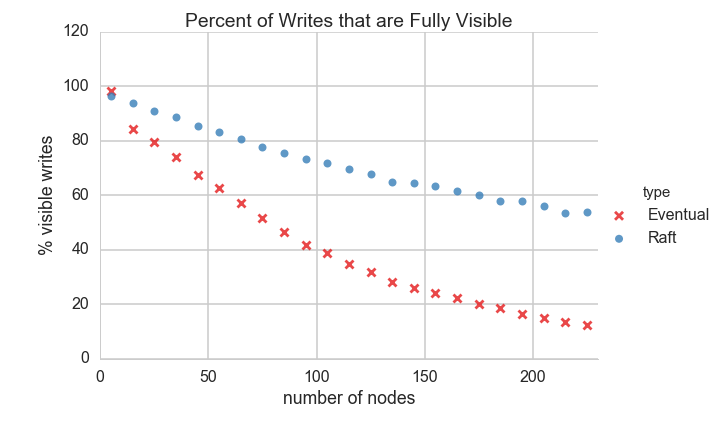
\includegraphics[width=\linewidth]{figures/scaling/visible_writes}
      \caption{Percent of fully visible writes in homogenous eventual and sequential consistency systems.}
      \label{fig:scaling_visible_writes}
    \endminipage\hfill
    \minipage{0.48\textwidth}
      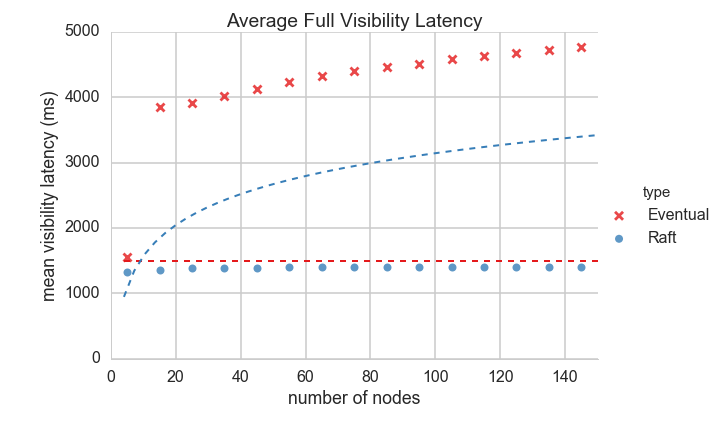
\includegraphics[width=\linewidth]{figures/scaling/visibility_latency}
      \caption{Latency of full visibility in homogenous eventual and sequential consistency systems.}
      \label{fig:scaling_visibility_latency}
    \endminipage
\end{figure*}

Because most research on gossip protocols and quorums specifies small quorums of a size that provide a minimum fault tolerance, our first question related to the effect of consistency protocols with increasing numbers of nodes. We created two homogenous distributed systems: an eventual consistency system implemented with anti-entropy via bilateral gossip and a latest-writer wins policy and sequential consistency by consensus implemented using the Raft consensus algorithm. Each simulation varied the number of nodes in one of five locations, e.g. 5 nodes had one node per location, 25 with 5 nodes per location, up to 100 with 20 nodes per location. Local area latencies were normally distributed with the mean latency, $\lambda_{\mu}=30$ms and the standard deviation of latency, $\lambda_{\sigma}=5$ms whereas wide area latencies were higher and more variable, $\lambda_{\mu}=300$ms and $\lambda_{\sigma}=50$ms.

The timing parameters for both Eventual and Raft are based on the network latency. We first computed a conservative timing parameter, $T=10\lambda_{\mu}$ based on the wide area latency mean. The anti-entropy interval for Eventual consistency is given as $\frac {T} {4} = 750$ms. For Raft, the heartbeat interval is $\frac {T} {2} = 1500$ms and the election timeout is a uniform random selection in the range $U(T, 2T) = U(3000, 6000)$. These conservative timing parameters ensure that it is rare that messages arrive out of order.

As the number of nodes increases, both Raft and Eventual systems start to degrade in terms of the percent of writes that are fully visible as shown in Figure \ref{fig:scaling_visible_writes}. For Eventual, this is because the time to visibility is related to the number of pairwise anti-entropy sessions required to propagate a write to all nodes as shown in Figure \ref{fig:scaling_visibility_latency}, where the blue line represents perfect convergence (not likely given uniform random neighbor selection). Raft on the other hand has a broadcast mechanism related to its heartbeat interval but writes do not become fully visible because they are rejected by the leader as inconsistent.

\begin{figure*}
    \centering
    \minipage{0.48\textwidth}
      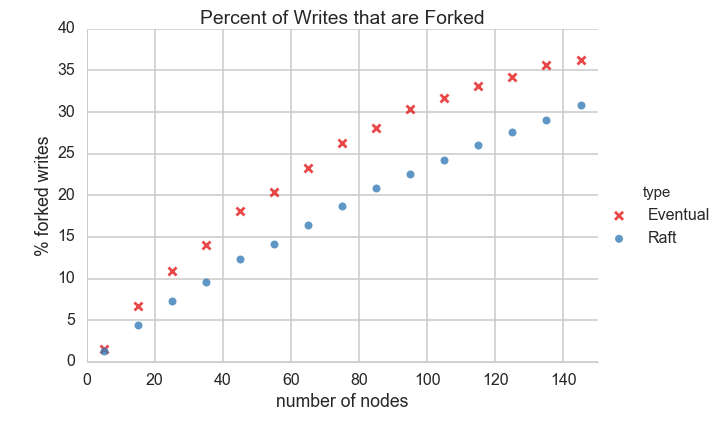
\includegraphics[width=\linewidth]{figures/scaling/forked_writes}
      \caption{Increasing forks in homogenous systems as topology size increases.}
      \label{fig:scaling_forked_writes}
    \endminipage\hfill
    \minipage{0.48\textwidth}
      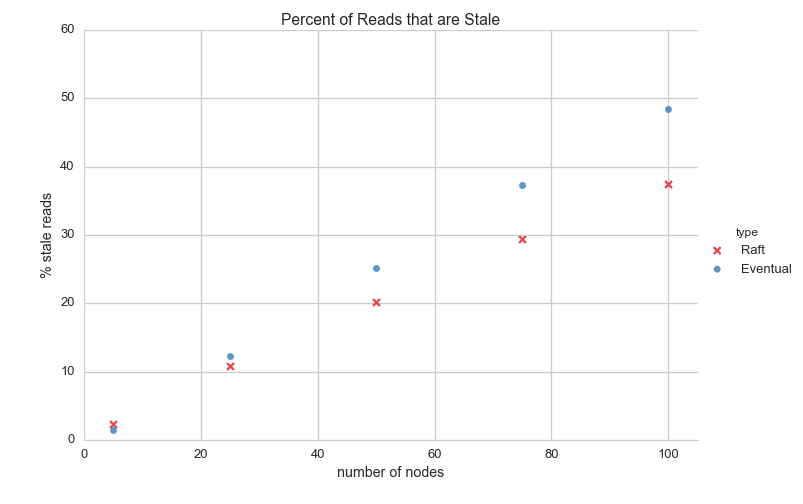
\includegraphics[width=\linewidth]{figures/scaling/stale_reads}
      \caption{Increasing stale reads in homogenous systems as topology size increases.}
      \label{fig:scaling_stale_reads}
    \endminipage
\end{figure*}

Read and write accesses were conducted on each device on 15 objects such that the probability of conflict, $P_c=0.3$ meaning that 30\% of the objects accessed on each device would also be accessed on another device. Accesses were issued at intervals normally distributed with the access interval mean, $A_{\mu}=3000$ms and the access interval standard deviation, $A_{\sigma}=380$ms such that accesses were roughly related to the timing parameter. As the number of nodes increases, the number of conflicts also increase, but not the likelihood of a conflict. Our system measures inconsistencies as \textit{forks} and \textit{stale reads}. As shown in Figure \ref{fig:scaling_forked_writes}, the number of conflicts in Raft is lower than in eventual as are the number of stale reads as shown in \ref{fig:scaling_stale_reads} but at the cost of a performance decrease, particularly as the number of nodes increases.

We believe that these initial investigations show a critical opportunity: that we can blend the high availability of an eventually consistent system and leverage the best parts of anti-entropy and eventual consistency in network environments where messages cannot get through along with the stability and increased visibility of a strongly consistent core, similar to the central core and flexible outer shell proposed by Gray and Oceanstore \cite{gray_dangers_1996,kubiatowicz_oceanstore:_2000}: we call this \textit{Federated Consistency}. Furthermore, if we can find a way to allocate decision space to a smaller number of nodes, we should be able to scale Raft to greater number of nodes without as steep a curve: we investigate this in \textit{Hierarchical Consensus}. Finally, as suggested by the $T$ timing parameter (though not explicitly covered), the timing measures and performance of consistency protocols are related to the network environment, which is dynamic. Potentially we can improve performance by monitoring the environment and adapting timing parameters to minimize the number of inconsistencies: investigated in \textit{Adaptive Consistency}.

\subsection{Topology}

In order to investigate the effect of variable latency and the network environment on consistency, we have constructed a fully connected topology of replica nodes that are each assigned a geographic region as shown in Figure \ref{fig:topology}. Within each region, replica nodes enjoy stable, low-latency connections with their neighbors. However, across regions the latency is higher and the connections variable, meaning that out of order messages are more common across the wide area than in the local area.

\begin{figure*}
    \centering
    \minipage{0.5\textwidth}
      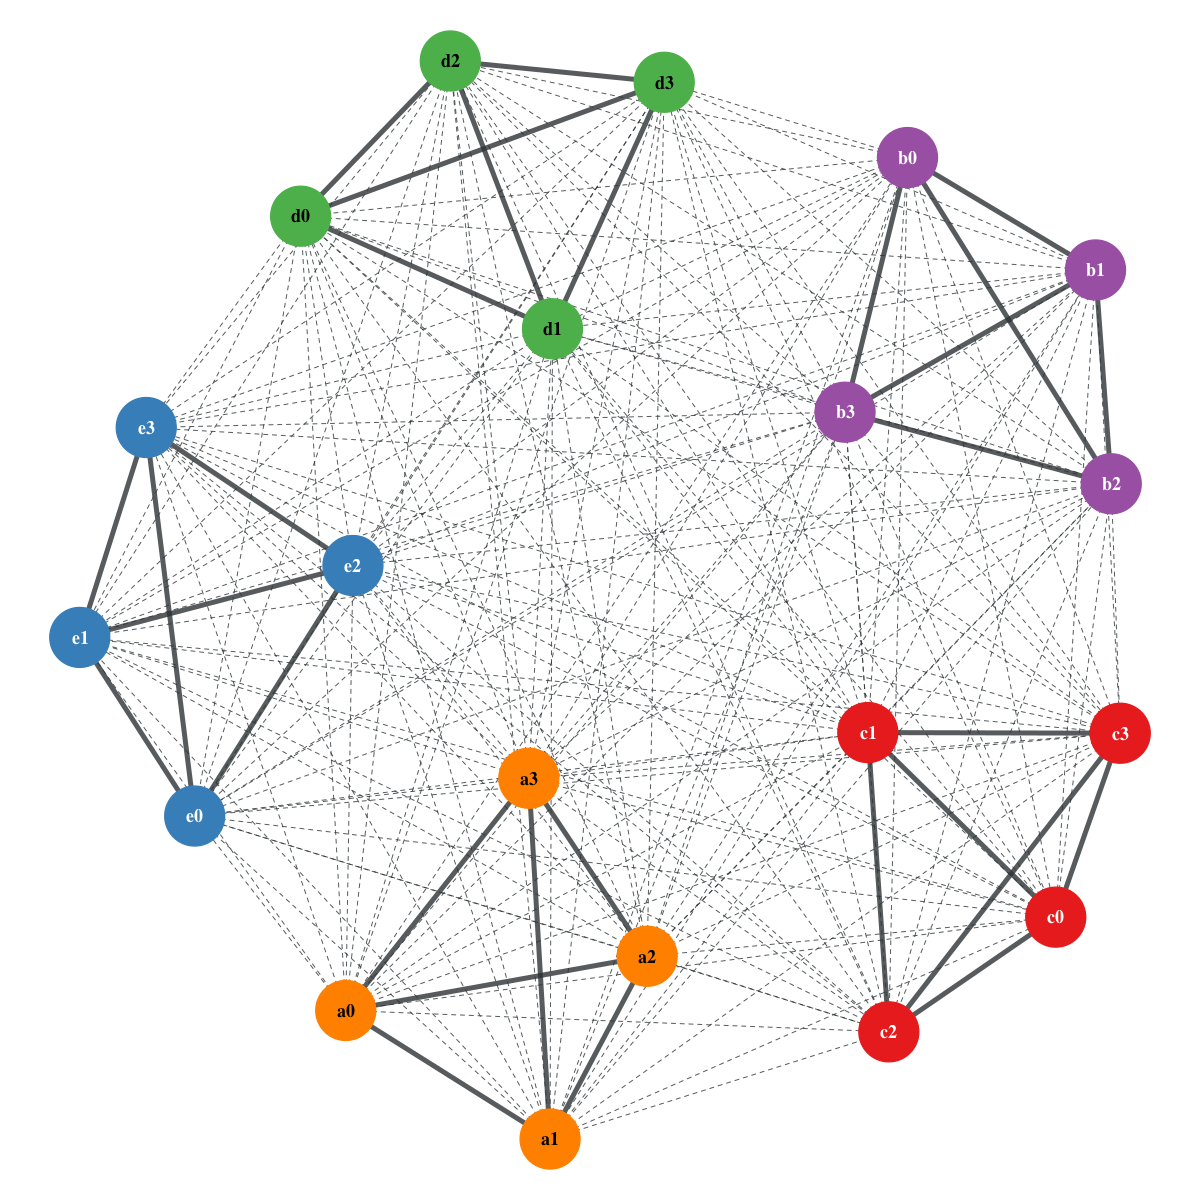
\includegraphics[width=\linewidth]{figures/topology}
      \caption{Proposed Network Topology.}
      \label{fig:topology}
    \endminipage\hfill
    \minipage{0.5\textwidth}
      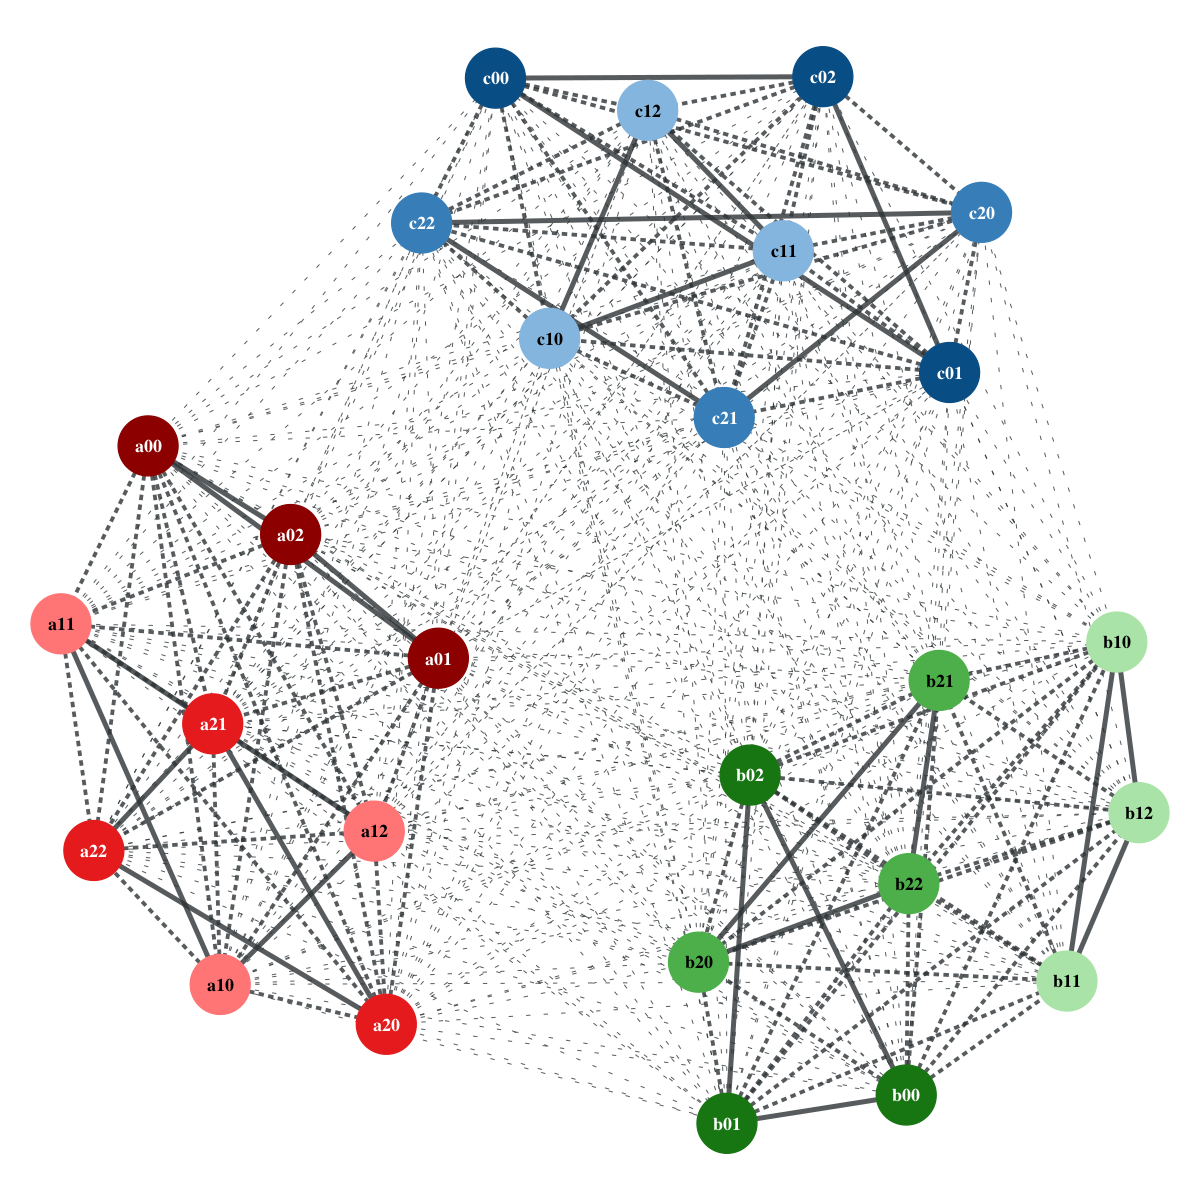
\includegraphics[width=\linewidth]{figures/tiers}
      \caption{Proposed Network Hierarchy.}
      \label{fig:tiers}
    \endminipage
\end{figure*}

In this type of topology there are two types of failure: node failure and network partitions. \textit{Node failure} occurs when a single node is shut off or stops responding to messages. \textit{Network partitions} occur when it is not possible for messages to be sent or received from a single geographic region. In both cases, two conditions must be dealt with by the replication protocol in order to satisfy correctness criteria: first the fact that accesses may continue at a partitioned node which are not being replicated by the system and second that the partitioned nodes are behind the global state and must be brought up to date.

For hierarchical consensus we have introduced a three tier topology consisting of three regions where nodes enjoy two types of network connections as shown in Figure \ref{fig:tiers}. Each region of nine nodes has three inner circles of very high connectivity (e.g. hard lines) while connectivity in the rest of the region is moderate and connectivity across the wide area is variable. This topology will allow us to explore hierarchical models in depth.

\subsection{System Description}

Our file system aggregates individual accesses into \textit{Close-To-Open} (CTO) consistency where read and write accesses are ``whole file'' \cite{muthitacharoen_low-bandwidth_2001}. Furthermore, with respect to local accesses we guarantee that a read returns the last write (given no remote updates, \textit{Read Your Writes Consistency}) and that writes are atomic with respect to each other (\textit{Monotonic Write Consistency}) \cite{bermbach_consistency_2013}.

Each replica's log is composed of a series of write accesses to multiple objects. Each object has a unique name that identifies it to the system and a monotonically increasing version number which can be implemented either as a vector clock \cite{parker_detection_1983} (or a simple Lamport scaler) in the case of a fixed topology or as a vector stamp \cite{almeida_version_2002} in the case of dynamic topologies. Therefore a write access encapsulate the following information: the name of the object being written to, the parent version of the object to which the write is being applied, the versions and object names of any other dependencies, the replica id where the write occurred, and an array of blob ids that compose the file at the conclusion of the write.

A read access to a particular object simply looks up the latest local version of that object. Because dependency information can be embedded into a write, it is not necessary to include read accesses in the log. For example, in order to create a transaction that reads from objects $X$ and $Y$, performs a computation then updates objects $Y$ and then $Z$: the write to $Y$ would include as a dependency the earlier version of $Y$ and the read version of $X$ and the write to $Z$ would include the updated version of $Y$ and the read version of $X$. Other notions of dependencies include implicit session dependencies, e.g. all writes are dependent on any access that occur within a minimum time threshold of each other, or explicit dependencies that are added by the application.

Because our system model accounts for heterogenous devices and each write in the log is simply metadata about the version of a file we consider version replication as a separate issue from object or blob replication. Furthermore, system consistency depends only on the replication of version information since a version defines what is visible on each replica to be read (and writes follow an implicit read). While a version must become visible (replicated to) all devices in order for the system to be consistent, the blobs that make up data may not be stored on all devices with different storage resources. If a read access requires blobs that it doesn't have, it can simply request them from a local neighbor that does, or from the origin replica itself.

\section{Proposed Work}

In order to investigate the effects of consistency and scaling in heterogenous, partition prone, variable latency networks we propose to build a distributed file system called FlowFS that implements two primary methodologies: Federated Consistency and Hierarchical Consensus. Federated Consistency allows us to create a flexible, heterogenous distributed system, allowing different replica servers to maintain different consistency levels based on need, but ensuring that global consistency guarantees are met. Hierarchical Consensus extends the Raft consensus protocol such that the quorum can scale, providing high availability sequential consistency. We further propose the stretch goal of the investigation of real time optimization and adaptation in response to changing network environments in mobile contexts. This stretch investigation will explore heuristic methods of optimization and steering configuration changes, as well as explore active, machine learning mechanisms

\subsection{Federated Consistency}

Heterogenous topologies with multiple users mean a variety of requirements for both availability and correctness. For example, consider a user working on a non-critical document on a train with limited cellular connectivity; the requirement here is probably high availability and progress rather than strong replication. On the other hand, during collaborative document editing, users might want to ensure strong sequential consistency and are willing to accept minimal delays such that the document is always in a consistent state. However, it is not possible to maintain a single, global consistency level that meets both of these requirements, leading us to the question: can consistency be adapted or tuned at runtime in such a way as to provide more availability in low connectivity situations or for low conflict objects and strong consistency and correctness in optimal network conditions or for critical or high priority workloads?

% Make sure to show that this is work already underway.

In order to scale a distributed storage system in the face of variable, partition-prone network environments and heterogenous, wide-area topologies

The Federated Consistency model allows individual replicas to select their own local consistency policies and engage in replication according to the mechanism specified by the policy. Each replica maintains its own local state which is modified in response to local accesses as well as the receipt of messages from remote replicas. Each replica sends messages to other nodes in order to propagate the latest writes as well as to perform housekeeping. Therefore every replica can be seen as an event handler that responds to local access events as well as remote messages and generates more events (sent messages) in return. Simply put, so long as every federated replica has an event handler for all types of RPC messages, federation only has to be defined at the \textit{consistency boundaries}, that is when replicas of one consistency type send messages to that of another.

Given the consistency models discussed in the previous section, we will omit weak consistency as being too simplistic and linearizability as being too performance restrictive. Instead we will focus on the federation of eventual consistency, implemented with latest-writer wins gossip based anti-entropy, and sequential consistency implemented with the Raft consensus algorithm.

A federated consistency protocol finds a middle ground in the trade-off between performance and consistency, particularly between an eventually consistent system implemented via gossip-based anti-entropy \cite{kempe_gossip-based_2003} and a sequential consistency model implemented by the Raft consensus protocol \cite{ongaro_search_2014}. By exploring these two extremes in the consistency spectrum we show that the overall number of inconsistencies in the system is reduced from the homogenous eventual system and that the access latency is decreased from the homogenous sequential system. Moreover, because the global consistency of the system is topology-dependent, it can be said to have flexible or dynamic consistency. We have found that large systems with variable latency in different geographic regions can perform well by allowing most nodes to operate in an optimistic fashion, but maintain a strong central quorum to reduce the amount of global conflict.

\subsubsection{Gossip and Anti-Entropy}

Eventual consistency is implemented by periodic \textit{anti-entropy} sessions that converge replicas towards the same state (e.g. reducing entropy, the divergence between the states of individual replicas) \cite{kempe_gossip-based_2003}. On a routine interval, specified by the \texttt{anti-entropy delay} timing parameter, a replica will randomly select one of the other replicas in the system and send a \texttt{Gossip} message that contains the latest version of all objects in the replica's local log. On receipt of the \texttt{Gossip} message, the remote replica will compare the RPC object versions with those in its local log. If the RPC versions are later, it will append the later versions of the object to the log (\textit{last-writer wins}). However if the remote object version is later it will send that version back to the originating node in a \texttt{GossipResponse} message. As a result, our anti-entropy implementation is \textit{bilateral}.

Replicas that implement eventual consistency read locally and write to their local latest version introducing zero read and write latency. Forks are caused by staleness due to the amount of time it takes to propagate a write to the rest of the system, the visibility latency.

\subsubsection{Strong Core Consensus Group}

Sequential consistency is implemented via the Raft consensus algorithm \cite{ongaro_search_2014}. However, consensus alone does not ensure that sequential consistency is implemented and a number of policy decisions about how Raft followers read and write and interact with the leader must be discussed.

The Raft leader has the primary responsibility of coordinating all other Raft replicas. To that end, the leader will broadcast periodic \texttt{AppendEntries} messages to all other Raft followers in order to maintain their leadership for the given term. A write access that originates at a follower must be sent as a \texttt{RemoteWrite} to the leader. The leader accepts writes in the order that they are received, and if the leader detects a fork -- that is that a write has a parent version who already has a child version in the log -- Raft will simply reject (drop) the write. In order to minimize the number of messages that Raft sends, Raft will aggregate all writes into the next \texttt{AppendEntries} message and send them together.

Because all writes that originate at followers are forwarded to the leader, the leader can guarantee a sequential ordering of updates. Therefore on receipt of an \texttt{AppendEntries} message, followers simply add the entries to their log and respond with their last index. If a majority of followers append entries to their logs, the leader will mark those entries as committed and inform the followers the write has been committed on the next \texttt{AppendEntries}.

However, although all writes are sequentially ordered, Raft nodes must decide what to do read, and there are several options:

\begin{enumerate}
    \item \textit{READ COMMITTED} Raft replicas will only read the latest committed version of an object, guaranteeing that the write will not be rolled back in the case of an outage. However, this read mode introduces the potential for a lot of staleness and therefore forks.
    \item \textit{READ LATEST} Raft replicas will read the latest version of the object in their log, even if it hasn't been committed. Moreover, replicas will read their own local writes rather than waiting for an \texttt{AppendEntries} to return their write.
    \item \textit{REMOTE READ} Rather than read locally, simply request the latest version from the leader. This introduces the potential for additional latency, but may be faster if the expected message latency is less than the heartbeat interval.
\end{enumerate}

Each of these options has critical implications for the likelihood of stale reads and writes in the system. Replicas would choose read committed if the network was highly partition prone and messages from the leader were unstable and prone to being rolled back. Remote read servers replicas well when the average message latency is far lower than the heartbeat interval, though this could be improved by making the heartbeat interval similar to the network latency. For this reason, we have selected read latest as the most likely scenario for a file system implementing sequential consistency with Raft.

\subsubsection{Integration}

A key requirement of Federated Consistency is the opportunity to create a homogenous systems with no performance cost, e.g. a homogenous eventual cloud and a homogenous Raft cloud will perform equivalently even if they implement the Federated protocol. However, if a strong, central consensus group is present, the eventual cloud should be able to synchronize with it, minimizing forks in the long run. Similarly, Raft nodes should be able to use anti-entropy mechanisms to replicate data and continue writing even if the leader is unavailable and no consensus can be reached to elect a leader.

Because anti-entropy messages have no implication on the state of consensus, we have elected to use 

\subsection{Hierarchical Consensus}

Federated consistency presents the opportunity to extend distributed storage systems to medium to large scale networks comprised of dozens of replica servers even in the face of high variability in unstable, mobile network environments. By allowing replicas to participate in eventual consistency replication if required to maintain a minimum quality of service, the system becomes flexible enough to handle variability. The key to Federation, however, is the strong central quorum that coordinates partitions in the eventual cloud, handling conflicts and pruning forked branches, minimizing overall inconsistency in the system.

Given the critical nature of the central quorum, particularly with quorum nodes distributed geographically to provide high availability to synchronization requests, a natural question arises: can the quorum scale to meet the availability needs of the Federated system as the topology grows?

% Note that Fast Paxos language says "avoid the leader and send directly to acceptors" providing two "paths" to consensus - fast and short. However, I have read other places that this is the equivalent of performing the propose phase in advance of the quorum decision, similar to Raft.
Raft and Paxos optimize the three phase consensus procedure (propose, accept, commit) of quorums by nominating a dedicated proposer, often called the leader or coordinator, who is solely allowed to make voting proposals thus staging the propose phase in advance of any consensus decisions via election. However, the leader is also a single point of failure, and most work in consensus protocols regards correctness and fault tolerance of a system given partitions that remove the leader from connecting to a majority of nodes. Additionally, in order to achieve linearizablity, every single access (including reads) must go through the leader, making the leader a bottleneck whose response performance creates a floor for the overall performance of the system. In order to scale consensus to larger systems, leadership must be addressed.

There are two primary approaches to increasing the availability of the leader in the literature: optimistic ``paths'' and multiple leaders. The former method, implemented in Fast Paxos \cite{lamport_fast_2006}, Egalatarian Paxos \cite{moraru_egalitarian_2012}, and S-Paxos \cite{biely_s-paxos:_2012} allows clients to directly contact acceptors (followers) with proposals, bypassing the leader and distributing leadership activities in a so called optimistic ``fast path''. However, in order to maintain correctness some conflict detection method is required; for example Fast Paxos requires larger quorums for fast path, and Egalitarian Paxos adds dependencies that are checked at ``execution'', where a dependency failure requires a fall back to the ``classic (slow) path''. The latter method allocates the decision space to multiple coordinators either by load balancing multiple quorums as in Multi-Paxos \cite{camargos_multicoordinated_2007} or by utilizing a per-tablet (a grouping of objects) quorum as in BigTable \cite{chang_bigtable:_2008}. Per-tablet quorums also reduce the likelihood of conflicts introducing the possibility of a hybrid approach: optimistic fast paths on multiple quorums with conflict detection and slow path resolution as in MDCC \cite{kraska_mdcc:_2013}.

Unfortunately these approaches, while working well on smaller scale quorum sizes (3-7 nodes), do not scale well in heterogenous and variable-latency environments. Fast-path requires optimism that conflict is relatively rare, otherwise it performs worse than simple classic-path methods since it must implement conflict detection. In larger networks, conflict is more likely, both because of the increased number of writers and owing to message delay. Allocating multiple, small quorums to different decision spaces requires that objects in different tablets be independent of each other; that is, there is no way to order writes sequentially to objects in tablets maintained by separate quorums. Federated consistency, however, requires a single, sequential ordering of all writes to maintain the eventual cloud and many applications of personal clouds that have implicit dependencies not easily embedded as application-level invariants, such as those specified database schemas.

We propose Hierarchical Consensus as a solution to scaling consensus to larger networks while still maintaining a sequential ordering across all objects such that dependencies between objects are determined at runtime. Our approach uses a tiered structure of leadership where the object namespace is governed by a root quorum that partitions the namespace to smaller subquorums via consensus decisions. This allocation creates an ordered set of epochs where each epoch defines a specific mapping of objects to subquorums such that all objects maintained by a single quorum are dependent on each other and \textit{on no other subquorum}. Every access that occurs in a single epoch is said to have \textit{happened before} every access in previous epochs, every write within a subquorum is ordered with respect to that quorum's decisions, and every write between quorums within a single epoch is said to be concurrent.

Hierarchical consensus therefore provides \textit{sequential consistency} on the entire namespace with accesses to objects whose dependencies may change over time. Hierarchical consensus is more available due to the use of multiple, smaller quorums and the localization of leadership to where accesses are occurring.

\subsubsection{Consensus Consistency}

Generalized consensus considers the problem of commands applied to a state machine in the same order. A distributed system of state machines is said to be consistent if all nodes have the same state within some reasonable delay and correct if the same exact sequence of commands was applied in the same order to reach the final state. The commands themselves generally have no dependencies and agreement considers no invariants beyond whether or not accepting the command would violate the consistency and correctness.

In order to implement a file system with generalized consensus, a couple of approaches can be taken. The most obvious approach is to use consensus to grant locks to replica, object pairs and unlocks once the write has been fully replicated. So long as read/write locks are observed, this system implements linearizeablity and is equivalent to two phase commit though such a system suffers from poor performance. Instead, the approach that we take is to make accesses the commands such that the state machine becomes an ordered series of accesses. If both read and write accesses are applied to the log (meaning that both a read and a write must be remote through the leader) then the system remains linearizable. However, in order to improve performance, we allow reads to occur to the local log of each follower, introducing the possibility of a fork if the local read is behind the global state and a write is submitted that modifies the stale read. Leaders must therefore check writes to ensure that they are not forked and drop those that are.

\begin{figure}
    \centering
        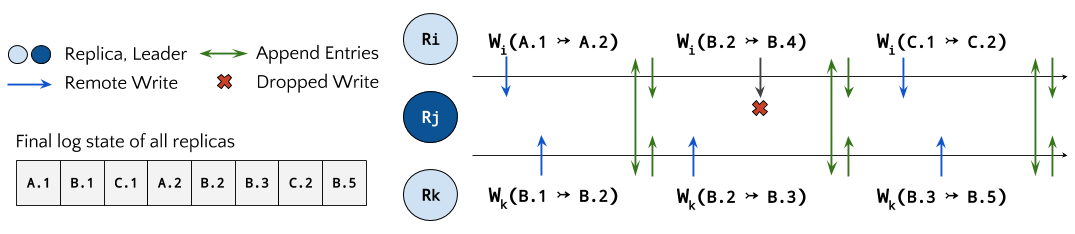
\includegraphics[width=.9\textwidth]{figures/ordered}
        \caption{Sequential ordering in consensus based file system}
        \label{fig:ordered}
\end{figure}

Consider the simple example shown in Figure \ref{fig:ordered}, implemented using the Raft protocol where writes are aggregated in \texttt{AppendEntries} (shown as green lines that occur routinely every heartbeat interval). In this example the object namespace is the set $\{A, B, C\}$ and each version is represented as the object name dot annotated with a monotonically increasing version number (we presume that version 1 of each object has already been written to the log). A write is conducted by reading the latest version of the object and writing the new version, therefore a write by replica $i$ that reads version $n$ and writes to version $m$ on object $O$ is given as follows: $W_i(O.n \rightarrowtail O.m)$.   Writes are ordered with respect to their arrival at the leader ($R_j$), are appended to the logs of the followers on \texttt{AppendEntries}, are committed by the leader when a majority of followers responds affirmative to the append RPC, and are marked as committed by followers on the subsequent \texttt{AppendEntries}. The leader must reject $W_i(B.2 \rightarrowtail B.4)$ in order to maintain consistency because that write would cause a fork to occur in the log. The final log is identically ordered on all replicas for all objects, therefore we can say we have achieved sequential consistency such that every write that appears in log position $i$ happens before ($\rightarrow$) the log entry at $i-1$.

In this example, we have only nominated one \textit{explicit} dependency on each write, the parent version, and enforced a no-forks invariant as a policy on this dependency at the leader. A consequence of this style consistency is the \textit{implicit} causality of all prior writes to a given write. For example, $W_i(C.1 \rightarrowtail C.2)$ implies implicit dependencies on $A.2$ and $B.3$, e.g. any versions that could have possibly been read prior to the write (and also the reason that reads must be logged in order to achieve linearizability). Similarly $W_k(B.3 \rightarrowtail B.5)$ has implicit dependencies on $A.2$ and $C.1$, more closely inspecting the log we can see that $C.2 \rightarrow B.5$ and $C.1 \rightarrow C.2$ therefore by transitivity, $C.1 \rightarrow B.5$, a correct interpretation of the log and implicit dependencies.

While implicit dependencies are critical to consistency, we observe that it is unlikely that a write is truly dependent on every historical write but is rather dependent on a local, recent subset of the namespace \cite{bailis_potential_2012}. Hierarchical consensus therefore makes use of \textit{explicit} causality to allocate the namespace to subquorums in order to balance the leader workload. This has several implications including allowing the ability to lock the ownership of a series of critical files, to specify particular replicas as stable storage for high value data, or to maintain policies and invariants that go beyond ordering; for example spatial polices (what data gets stored), temporal policies (what versions are stored) and synchronization policies (how and when replication occurs).

\subsubsection{Namespace Allocation}

\begin{figure}
    \centering
        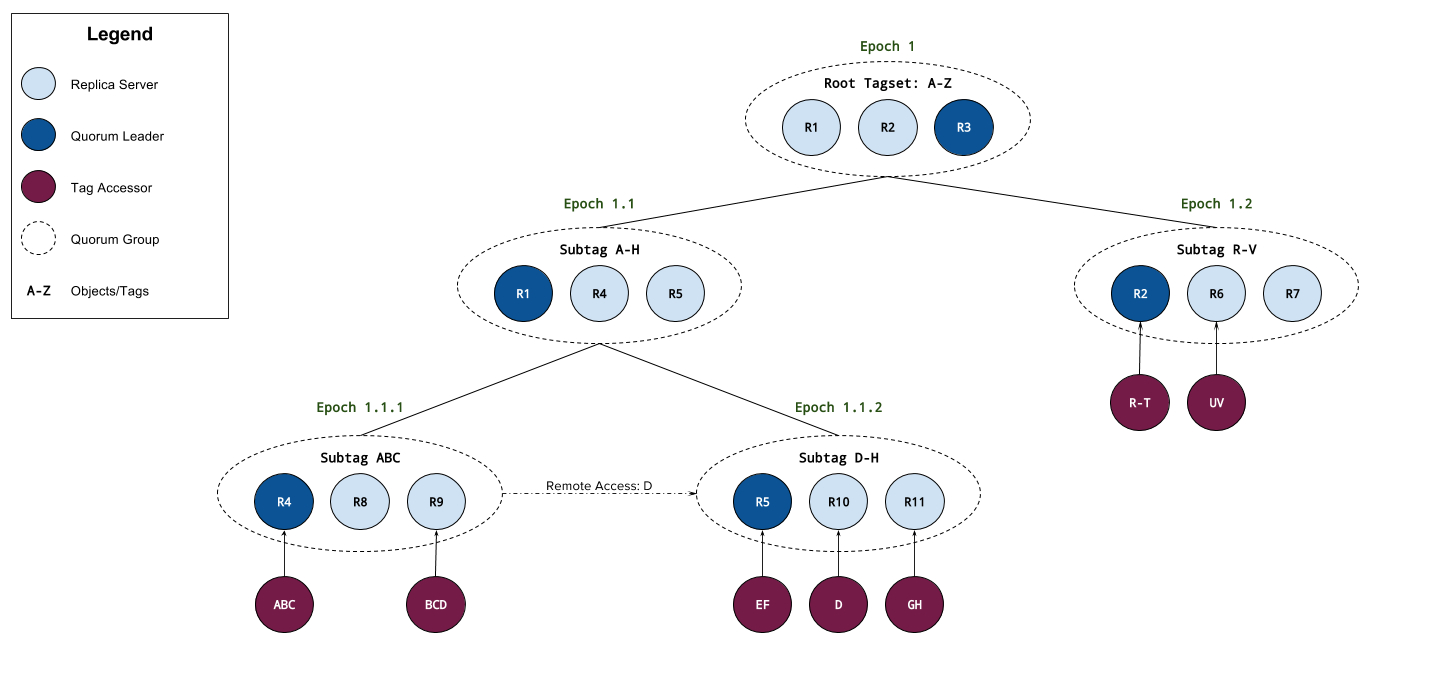
\includegraphics[width=.9\textwidth]{figures/hierarchical}
        \caption{Hierarchical consensus partitions the namespace across subquorums}
        \label{fig:hierarchical}
\end{figure}

An open question for our research is how to automatically allocate the namespace such that leadership of a subset of the namespace is local to the accesses and that members of the quorum are distributed to provide wide area durability and availability. The goal of allocation, is shown in Figure \ref{fig:hierarchical} - a hierarchy of quorums such that the children of each tier manage consensus decisions on a non-overlapping portion of the namespace.

Consider a motivating example using the notion of \textit{sessions}. Starting from a quiescent state (no accesses), a node or a group of nodes begins reading and writing to a set of objects (perhaps collaborative editing of a document, or a series of financial transactions); we expect that after some finite amount of time, the access pattern will change or cease. We can therefore state that all objects involved in a single session are explicitly causally related to each other and to no other objects in the namespace. Whether we describe sessions as a fixed, sliding window or as something more variable, some automatic determination that those objects should be coordinated together is necessary. To that end we will define a \textit{tag} as a time-annotated subset of the namespace and a \textit{tagspace} as the set of non-overlapping tags that compose the namespace for a given time period.

Hierarchical consensus starts with a root quorum whose responsibility is to govern the entire namespace. The root quorum does so by maintaining a root \textit{epoch}, a monotonically increasing counter which identifies the current \textit{tagspace}. In addition to consensus decisions related to leader election, accesses, and membership changes, decisions that modify the tagspace also require consensus. We define two primary operations: \textit{split} creates a new subquorum, splitting a larger tag from the previous tagspace and \textit{join} removes a subquorum, joining two smaller tags from the previous tagspace. Any decision that modifies the tagspace (thus creating a new tagspace) requires an increment of the \textit{epoch}.

The fundamental relationship between accesses in epochs is as follows: any access that happens in epoch $i$ happened before every access in epoch $i-1$; accesses in different tags but in the same epoch happen concurrently from the global perspective, but are ordered locally in the quorum that governs that tag. As a result, every log has a determined, sequentially consistent and correct ordering, though the logs of two individual replicas may differ. Hierarchical consensus cannot provide linearizability, but does provide sequential consistency.

\subsubsection{Operation}

\begin{figure}
    \centering
        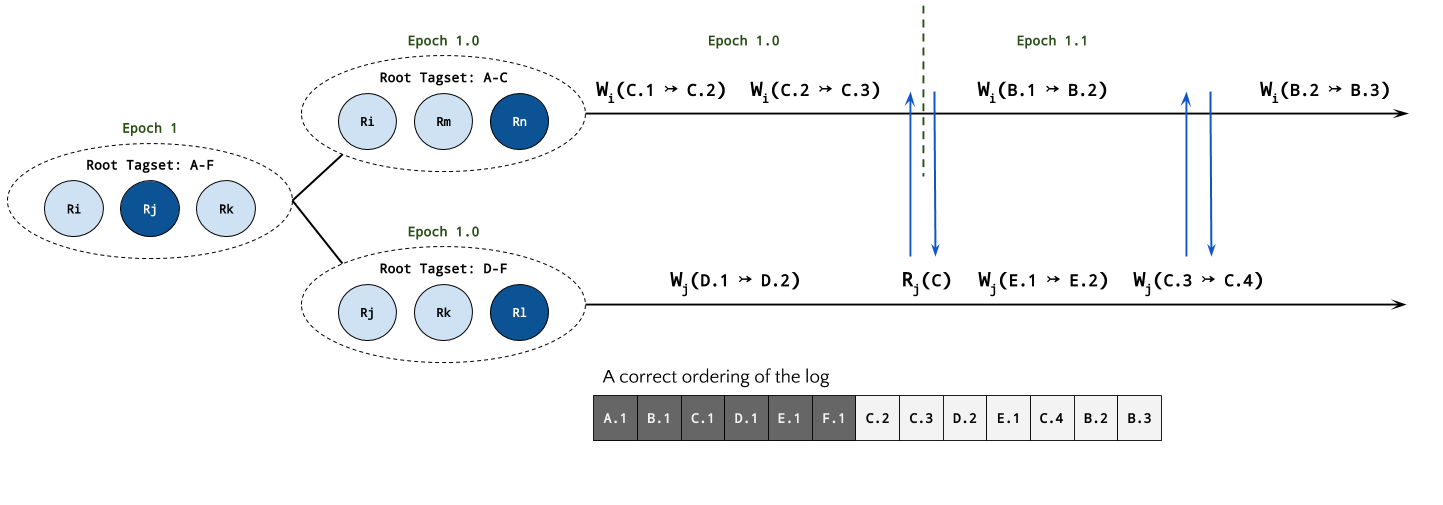
\includegraphics[width=.9\textwidth]{figures/subepoch}
        \caption{Sub-epochs allow remote accesses between tags without a tagspace change.}
        \label{fig:subepoch}
\end{figure}

The namespace allocation creates a tiered structure of leadership such that the root quorum is responsible for the entire namespace, subquorums are responsible for tags, and leaves are responsible for handling accesses to their tag. Any access to an object must be forwarded as a remote access to the leader of the quorum that handles the tag that encapsulates the object. The only exception is the optimization made for members of the quorum who can read locally any object in their tag space. By optimizing the locality of access and spreading the workload to multiple leaders, we hope to show that the overall performance of the system increases.

When a member of a quorum wishes to access an object that is not in that quorum's tag, one of two things must happen: either a tag decision must be made to reallocate the tag space such that it is local to the new accessor or some mechanism must allow remote accesses between quorums. The former case is expensive, but if the accesses to that object become routine then the upfront cost will pay for future accesses. However, for non-routine accesses some mechanism for remote access is required.

The issue is that a remote access from one tag to another creates an implicit dependency between all accesses that happened before the remote access and all those that follow the local one. Correctness is maintained by the ordering of epochs, so some local split is required. Consider the example in Figure \ref{fig:subepoch}: the remote read access, $R_j(C)$ implies any writes to tag $D-F$ following the read depends an all writes in tag $A-C$ that occurred before the read. Furthermore, the remote write $W_j(C.3 \rightarrowtail C.4)$ is a non-conflicting write, depends on all writes on tag $D-F$ that happened before \textit{and} depends on all writes in tag $A-C$ that occurred before the remote read, and occurs concurrently with any writes that happen after so long as there is no conflict.

Our proposed solution is similar to the epoch solution: each tag quorum maintains a per-epoch, monotonically increasing sub-epoch counter. In the case of a remote access, that counter is incremented to demarcate the ordering of all accesses in the tag that happened before the remote access and all those that follow. This counter must be replicated in addition to the version number, and can therefore be seen as an explicit dependency applied to all remote writes. As a result, any quorum that receives these ordering indicators can appropriately order their logs.

This mechanism also leads us to suspect that generalizing the consensus hierarchy to arbitrarily deep levels is possible; particularly since the notion of sub-epoch numbers already exists. Clearly some coordination is required to ensure that tag space changes filter down to all leaf nodes, and that is the primary subject of our future work related to this proposal.

In addition to correctness, we also propose to show failure tolerance by utilize Raft-style quorum mechanics. There are two distinct kinds of failure in a hierarchical system: replica failures (a single node crashes and dies) and partitions, where parts of the network are cut off from receiving messages. We believe that we can model failure tolerance from both of these perspectives through a formulation of quorum size, minimal intersection set between quorums, and the depth/breadth of the hierarchy. We propose to show correctness in the face of failure in the least and will stretch to show inherent robustness due to the structure of the hierarchy.

\subsection{Adaptive Consistency}

Given the federation of multiple consistency models and the improved performance of consensus via hierarchical agreement, I propose the final step is the real time adaptation of the network according to observed latency values. Eventually consistent nodes can change their timing parameters at will to take advantage of lower latencies or to save work in sparse network conditions. Joint consensus is required to adapt the parameters of a consensus group. Machine learning algorithms can be used to further learn from the environment and optimize consistency guarantees.

\section{Timeline}

In order to meet the requirements of this proposal and provide substantive results for a dissertation, we propose to undertake the following projects, along with their given priority and timeline.

\begin{center}
\begin{tabular}{|l c|c|}
\hline
Project & Priority & Time Estimate \\
\hline
Simulation of Federated Consistency & $\bigtriangleup$ & 1 months \\
Simulation of Hierarchical Consensus & $\bigtriangleup$ & 2 months \\
Implementation of the FlowFS & $\bigtriangleup$ & 3-4 months \\
Evaluation of FlowFS on real workloads & $\bigtriangleup$ & 2-3 months \\
Proof of correctness and consistency & $\bigtriangleup$ & 1 month \\
Heuristics to optimize and allocate FlowFS & $\bigtriangledown$ & 1 month \\
Online optimization and consistency adaptation & $\bigtriangledown$ & 2-3 months \\
\hline
\multicolumn{2}{|l|}{\textbf{TOTAL}} & 12-16 months \\
\hline
\end{tabular}
\end{center}

After investigations and evaluations of Federated Consistency and Hierarchical Consensus in simulation, I propose to implement a file system utilizing both mechanisms and verify the system meets consistency requirements on large networks in real world workflows. Goals marked with $\bigtriangleup$ indicate necessary checkpoints to the successful completion of the dissertation, including some proof of correctness. I further propose the stretch goals (marked with $\bigtriangledown$) of real time adaptation and online optimization, investigating the application of both heuristics and active machine learning techniques to learn usage patterns and improve consistency and performance.

Based on preliminary work done in simulation I propose the following paper deadline goals:

\begin{itemize}
\item IEEE International Conference on Distributed Computing Systems, June 2017: Federated Consistency
% http://icdcs2017.gatech.edu/
\item ACM Hot Topics in Storage and File Systems 2017, July 2017: Personal Clouds
% https://www.usenix.org/conferences
\item ACM Principles of Distributed Computing, July 2017: Hierarchical Consensus
% http://www.podc.org/
\end{itemize}

\section{Conclusion}

Insert conclusion here.

\newpage

\appendix
\section{Appendix A: Reading List}
\label{app:readinglist}

\subsection{Consensus}

1) \bibentry{thomas_majority_1979}

2) \bibentry{lamport_paxos_2001}

3) \bibentry{chandra_paxos_2007}

4) \bibentry{lamport_fast_2006}

5) \bibentry{ongaro_search_2014}


\subsection{Consistency}

1) \bibentry{lamport_time_1978}

2) \bibentry{terry_managing_1995}

3) \bibentry{bailis_quantifying_2014}

4) \bibentry{bailis_potential_2012}

5) \bibentry{bermbach_consistency_2013}


\subsection{Replication}

1) \bibentry{stoica_chord:_2001}

2) \bibentry{kubiatowicz_oceanstore:_2000}

3) \bibentry{gray_dangers_1996}

4) \bibentry{venkataramani_operating_2002}

5) \bibentry{almeida_version_2002}



% \newpage

% \section{Appendix B}
% \label{app:cvtdp2r}


\newpage

\bibliographystyle{plain}
\bibliography{prelim}

\end{document}
